\documentclass{article}

\usepackage{amsmath}
\usepackage{amssymb}
\usepackage{graphicx}
\usepackage{hyperref}
\usepackage{xcolor}
\usepackage{listings}
\graphicspath{ {images/} }
\setlength\parindent{0pt}

\lstset{frame=tb,
	language=C++,
  	aboveskip=4mm,
  	belowskip=12mm,
  	showstringspaces=false,
  	columns=flexible,
  	basicstyle={\small\ttfamily},
  	numbers=none,
  	numberstyle=\tiny\color{gray},
  	keywordstyle=\color{blue},
  	commentstyle=\color{brown},
  	stringstyle=\color{red},
  	breaklines=true,
  	breakatwhitespace=true,
  	tabsize=4
}


\title{
	\Huge
	{Building a 3-D Physics Engine to Model Projectile Motion}\\
}
\author{Maxim Webb}

\begin{document}

\maketitle

\newpage

\begin{abstract}
This report will describe the process of building a 3-D physics engine, with the end goal being to create an accurate model for projectile motion.
\newline
\newline
However, this is not the sole goal; the aim throughout the project is to build a physics engine from first principles, without relying on pre-existing 3-D graphical APIs such as OpenGL, or Direct3D. Therefore, the report will also describe the mathematics behind the rendering process, as well as the necessary methods for representing 3-D transformations.
\newline
\end{abstract}
\newpage
\tableofcontents

\newpage

\section{Technology}
The program will be written in C++, for its speed, and for its object orientation, which will prove useful for the structure of the project. This includes the use of several template classes from the STL, such as \verb|<cmath>| and \verb|<vector>|.
\newline
\newline
Windows GDI will be used for basic graphical output, which is limited to drawing lines and polygons. 
\newline
\newline
Git will be used for this project, providing versatile and powerful VCS. The project's source code is available 
\href{https://github.com/maximwebb/3D-engine}{\color{blue} on Github}\color{black}.

\newpage
\section{Basic Structure}

First, the Point class will be the building blocks of the engine, with the parameter \verb|abs_pos| describing the absolute position in the universe. The method \verb|update()| will be fleshed out later.
\begin{lstlisting}
class Point {
public:
	/* Parameters */
	vector<float> abs_pos;
	
	void update() {
	
	}

}
\end{lstlisting}

Next, the Plane class stores an array of points, and contains a method for updating them iteratively. 
\begin{lstlisting}
class Plane {
public:
	/* Parameters */
	vector<Point> points;
	
	void update_points() {
		for (int p = 0; p < points.size(); p++) {
			points[p].update();
		}
	}
	
}
\end{lstlisting}
\newpage
The Obloid class is the umbrella class for all 3-D objects in the program. Obloids will take four points as parameters, and generate the remaining four vertices. From this, six planes (faces) can be constructed, and stored in an array. 
\newline
\newline
Obloids will also store physical attributes, such as mass and velocity, which will be added later.

\begin{lstlisting}
class Obloid {
public:

	/* Parameters: Top-Right-Front, Top-Right-Back, Bottom-Left-Back, Bottom-Left-Front */
	Point trf{ { 0, 0, 0, 1 } };
	Point trb{ { 0, 0, 0, 1 } };
	Point blb{ { 0, 0, 0, 1 } };
	Point blf{ { 0, 0, 0, 1 } };
	
	/* Generate remaining four vertices */
	Point brf{ { blb.abs_pos[0], trf.abs_pos[1], trf.abs_pos[2], 1 } };
	Point brb{ { blb.abs_pos[0], trf.abs_pos[1], blb.abs_pos[2], 1 } };
	Point tlf{ { trf.abs_pos[0], blb.abs_pos[1], trf.abs_pos[2], 1 } };
	Point tlb{ { trf.abs_pos[0], blb.abs_pos[1], blb.abs_pos[2], 1 } };
	
	/* Generate six planes */	
	Plane pl_top{ { trf, trb, tlb, tlf } };
	Plane pl_bottom{ { brf, brb, blb, blf } };
	Plane pl_left{ { tlf, tlb, blb, blf } };
	Plane pl_right{ { trf, brf, brb, trb } };
	Plane pl_front{ { trf, tlf, blf, brf } };
	Plane pl_back{ { trb, tlb, blb, brb } };
	
	vector<Plane> faces = { pl_left, pl_right, pl_bottom, pl_top, pl_back, pl_front };
	
	void update_faces(HDC hdc) {
		for (int f = 0; f < faces.size(); f++) {
			faces[f].update_points();
		}
	}
}
\end{lstlisting}

\newpage

The \verb|PLAYER| class will store global information about the viewer, including the viewer's position, velocity, field of view, and various other properties:

\begin{lstlisting}
class PLAYER {
public:

	/* Stores player's absolute universal coordinates from origin. */
	vector<int> coords = { 0, 0, 0 };
	vector<int> vel = { 0, 0, 0 };

	float fov = 120;	

};

PLAYER Player;
\end{lstlisting}

These four classes make up the fundamental structure of the program, and they will all be added to shortly.

\newpage
\section{Projecting onto the viewport}
When considering displaying objects on the viewport (the visible section of the screen), it becomes evident that a method is required for converting between the 3-D coordinates of the universe, and the 2-D coordinates of the viewport. This process must account for depth, thereby providing perspective.

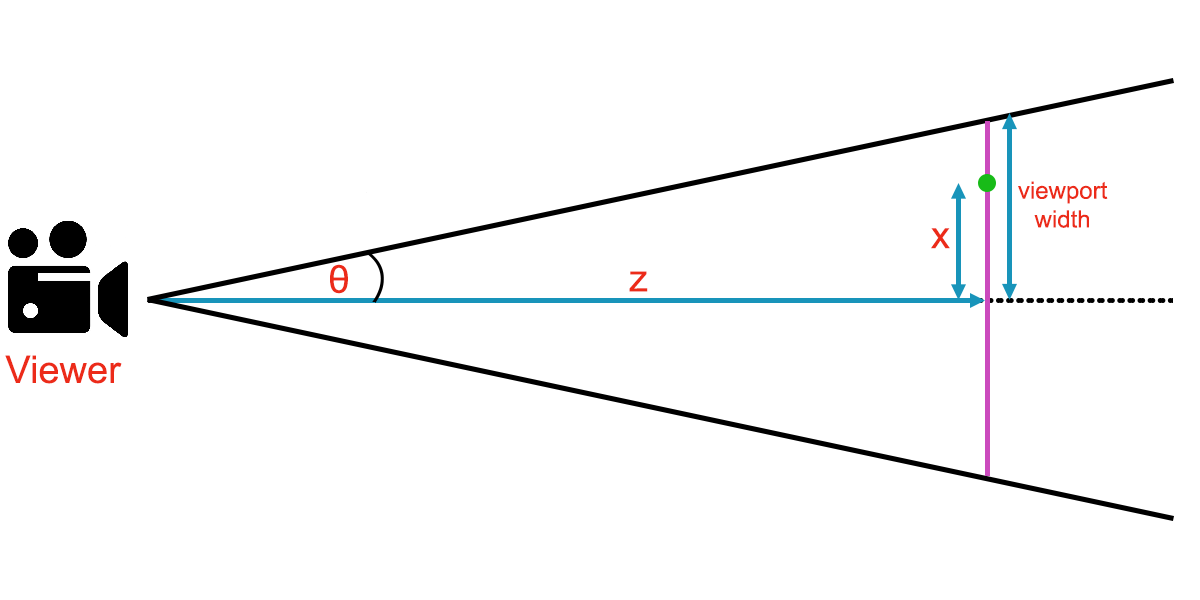
\includegraphics[width=1\textwidth]{projection_diagram.png}

The diagram shows a bird's eye view of the viewer's vision. The green dot represents a point in the viewer's line of sight, and is a certain z-distance away from the viewer. At this z-distance, there is a virtual plane to project the point onto, represented by the pink line. 
\newline
\newline
Then, the width of the virtual plane, and the ratio of this width to the point's displacement from the centre line is found as follows:
\newline
\newline
Let p = plane width, let x, z be coordinates of point:
$$ p = ztan{\theta} $$
$$ ratio = \frac{x}{ztan{\theta}} $$
Applying the same logic, the vertical ratio is $ \frac{y}{ztan{\theta}} $
\newline
\newline
Then, if the screen has width w and height h, the coordinates on the window $(s_x, s_y) $ are as follows:

$$ s_x = \frac{1}{2}w + \frac{xw}{ztan{\theta}} $$
$$ s_y = \frac{1}{2}h + \frac{yh}{ztan{\theta}} $$
\newpage
It is worth noting at this point that this method only works if the viewer is centred about (0, 0, 0). Therefore, in the Point class definition, there should be a second position coordinate, relative to the viewer. With this new type of coordinate, \verb|update()| can now be defined as shown:

\begin{lstlisting}
class Point {
public:
	/* Parameters */
	vector<float> abs_pos;
	
	vector<float> rel_pos;
	int screen_x;
	int screen_y;	
	
	void update() {
		screen_x = window_width * 0.5 + window_width * rel_pos[0] / (rel_pos[2] * tan(fov));

		screen_y = window_height * 0.5 + window_width * rel_pos[1] / (rel_pos[2] * tan(fov));
	}
	
	void draw(HDC hdc) {
	
	}
}

\end{lstlisting}
For clarity's sake, some of the variables have been renamed in the code, but the function is the same as the previous result.

\newpage

\section{Transformations of 3-D space}
Now that projections onto the viewport has been implemented, there needs to be a way of the viewer moving around the universe. This requires translating and rotating the universe about the viewer.
\newline
\newline
There are several methods for handling these transformations - one approach would be the use of quaternions, which are an extension of complex numbers, consisting of four separate parts to handle rotations. For this project, however, matrices will handle all transformations, predominantly for their versatility and speed in manipulating vector space.
\newline
\newline
The first problem to tackle is creating a matrix data type - C++ does not natively support matrices, so they will need to be built in manually. By using a typedef to define a \verb|matrix| data type as a nested array of floats:

\begin{lstlisting}
using matrix = vector<vector<float>>;
\end{lstlisting}

A function can be created that will take an array of 16 numbers and return a 4x4 matrix:
\begin{lstlisting}
matrix Mat(vector<float> arr) {
	matrix mat;

	for (int row = 0; row < 4; row++) {
		mat.push_back({});
		for (int col = 0; col < 4; col++) {
			mat[row].push_back(arr[row * 4 + col]);
		}
	}
	return mat;
}
\end{lstlisting}

While this approach may seem more convoluted than simply defining a matrix class, it allows for direct interaction with the elements inside the matrix, and is more lightweight than a class or struct.
\newline
\newline
Next, by defining matrix multiplication, it is possible to chain transformations and apply transformations to vectors. Here, the \verb|multiply()| function is overloaded so that multiplication between two matrices and multiplication between a matrix and a vector is separate. While this could be combined into a single function, it would require conversion of position vectors (currently 1-D arrays) into matrices (2-D arrays) each cycle, which is a computationally expensive process.

\begin{lstlisting}

/* Multiplies two matrices and returns the resulting matrix */
matrix multiply(matrix mat1, matrix mat2) {
	matrix mat3;
	for (int row = 0; row < 4; row++) {
		mat3.push_back({});
		for (int num = 0; num < 4; num++) {
			mat3[row].push_back(0);
			for (int col = 0; col < 4; col++) {
				mat3[row][num] += (mat1[row][col] * mat2[col][num]);
			}
		}
	}

	return mat3;
}

/* Multiplies a vector by a matrix and returns the resulting vector */
vector<int> multiply(matrix transform_mat, vector<int> pt) {
	vector<int> pt2;
	for (int row = 0; row < 4; row++) {
		pt2.push_back(0);
		for (int col = 0; col < 4; col++) {
			pt2[row] += (pt[col] * transform_mat[row][col]);
		}
	}

	return pt2;
}
\end{lstlisting}
\newpage

You may have noticed that all of the vectors and matrices defined thus far have been four dimensional, whereas the universe has only three spatial dimensions. The reasoning behind this is that whilst 3 x 3 matrices can be used to represent linear transformations, they cannot represent a translation, without defining an addition function.
\newline
\newline
Instead, by using four rows and columns, the (x, y, z) offset can be represented in the fourth column of the matrix as shown:

$$
M = 
\begin{pmatrix}
	1 & 0 & 0 & x \\
	0 & 1 & 0 & y \\
	0 & 0 & 1 & z \\
	0 & 0 & 0 & 1
	
\end {pmatrix}
$$

By storing the (x, y, z) offset as such, translations are kept separate of rotations, simplifying the process greatly. Translations are now defined by adding the player velocity vector to these entries in the matrix.
\newline
\newline
The rotation matrices can now be defined. For rotations about the y-axis:

$$ R_y = 
	\begin{pmatrix}
		\cos{\theta} & 0 & \sin{\theta} & 0 \\
		0 & 1 & 0 & 0 \\
		-\sin{\theta} & 0 & \cos{\theta} & 0 \\
		0 & 0 & 0 & 1
	\end{pmatrix}
$$
The matrix for rotations about the x-axis:
$$ R_x = 
	\begin{pmatrix}
		0 & 0 & 1 & 0 \\
		0 & \cos{\theta} & -\sin{\theta} & 0 \\
		0 & \sin{\theta} & \cos{\theta} & 0 \\
		0 & 0 & 0 & 1
	\end{pmatrix}
$$
And for the sake of completeness, rotations about the z-axis (this one will not be used, as it does not result in a particularly useful transformation).
$$
R_z = 
	\begin{pmatrix}
		\cos{\theta} & -\sin{\theta} & 0 & 0 \\
		\sin{\theta} & cos{\theta} & 0 & 0 \\
		0 & 0 & 1 & 0 \\
		0 & 0 & 0 & 1
	\end{pmatrix}
$$

\newpage
The \verb|pos| property for the Player class will be the matrix describing the current linear transformation of vector space: 

\begin{lstlisting}
class PLAYER {
public:

	/*Stores player's absolute universal coordinates from origin.*/
	vector<int> coords = { 0, 0, 0 };
	vector<int> vel = { 0, 0, 0 };


	float fov = 120;	
	
	matrix pos = Mat({ {1, 0, 0, 0,
					0, 1, 0, 0,
					0, 0, 1, 0,
					0, 0, 0, 1} });

};
\end{lstlisting}

These are all the necessary methods required to transform 3-D space, allowing the viewer to move and look around freely. In the next section, the necessary methods for updating and drawing the universe are detailed.
\newpage

\section{Updating and Drawing in the Event Loop}

Now that all of the fundamental groundwork is in place, there needs to be a graphical output. This is done by adding the following code to the plane class, meaning the quadrilateral defined by the plane's vertices will be filled in:

\begin{lstlisting}

class Plane {
public:
	/* Parameters */
	vector<Point> points;
	
	/* Other */
	POINT arr[4];
	
	void update_points() {
		for (int p = 0; p < points.size(); p++) {
			points[p].update();
			
			arr[i].x = points[i].screen_x;
			arr[i].y = points[i].screen_y;
		}
	}
	
	void fill_plane(HDC hdc) {	
		SelectObject(hdc, GetStockObject(DC_BRUSH));
		SetDCBrushColor(hdc, RGB(200, 35, 16));
		Polygon(hdc, points, 4);
	}
	
}
\end{lstlisting}

Note: \verb|arr| is a C-style array, used because the \verb|Polygon()| method requires a static array. Some code has been excluded from this section, but it is predominantly used for configuring Windows GDI, and is not relevant to the project.
\newpage
Adding \verb|fill_plane()| to the Obloid class's update loop, and defining a new Obloid, means that objects can now be drawn:

\begin{center}
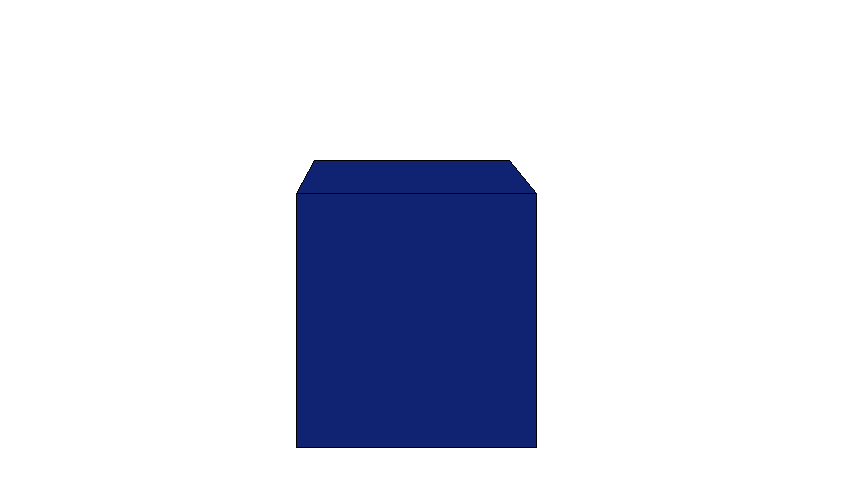
\includegraphics[width=0.5\textwidth]{first_cube.png}
\end{center}

Success! Next, in order to move and look around in the universe, an event loop is required. This will continuously update and draw all the objects in the universe:

\begin{lstlisting}

void clear(HDC hdc, RECT* prc) {
	HBRUSH brush_white = CreateSolidBrush(RGB(255, 255, 255));
	FillRect(hdc, prc, brush_white);
	DeleteObject(brush_white);
}

int timer = SetTimer(hWnd, MYTIMER, 5, NULL);

LRESULT CALLBACK WndProc(HWND hWnd, UINT message, WPARAM wParam, LPARAM lParam)
{
	//Above code hidden
	
	case WM_TIMER:
	{
	
		/* Checks for keyboard input & adjusts velocity */
		if (GetAsyncKeyState('A') < 0) {
			player.vel[0] = -5;
		}
		else if (GetAsyncKeyState('D') < 0) {
			player.vel[0] = 5;
		}
		
		else {
			player.vel[0] = 0;
		}

		if (GetAsyncKeyState('W') < 0) {
			player.vel[2] = 5;
		}
		else if (GetAsyncKeyState('S') < 0) {
			player.vel[2] = -5;
		}
		else {
			player.vel[2] = 0;
		}

		if (GetAsyncKeyState(0x20) < 0) {
			player.vel[1] = 5;
		}
		else if (GetAsyncKeyState(0xA0) < 0) {
			player.vel[1] = -5;
		}
		else {
			player.vel[1] = 0;
		}
		
		/* Updates viewer pos matrix */
		player.pos[0][3] += player.vel[0];
		player.pos[1][3] += player.vel[1];
		player.pos[2][3] += player.vel[2];
		
		clear(hdc, &window_rect);
		cube_1.update_faces(hdc);
		
\end{lstlisting}
Then, adding the rotation matrices from the previous section, the viewer can now freely look around the universe:

\begin{lstlisting}
	/* Keyboard input for rotations */
	if (GetAsyncKeyState(0x25) < 0) {
		player.x_ang = 0.025;
	}
	else if (GetAsyncKeyState(0x27) < 0) {
		player.x_ang = -0.025;
	}

	else {
		player.x_ang = 0;
	}
	if (GetAsyncKeyState(0x26) < 0) {
		player.y_ang = 0.025;
	}
	else if (GetAsyncKeyState(0x28) < 0) {
		player.y_ang = -0.025;
	}

	else {
		player.y_ang = 0;
	}

	matrix rot_x_mat = Mat({ { cos(player.x_ang), 0, sin(player.x_ang), 0,
		0, 1, 0, 0,
		-sin(player.x_ang), 0, cos(player.x_ang), 0,
		0, 0, 0, 1
		} });

	matrix rot_y_mat = Mat({ { 1, 0, 0, 0,
		0, cos(player.y_ang), sin(player.y_ang), 0,
		0, -sin(player.y_ang), cos(player.x_ang), 0,
		0, 0, 0, 1
		} });

	player.pos = multiply(rot_x_mat, player.pos);
	player.pos = multiply(rot_y_mat, player.pos);
\end{lstlisting}
Example of a working rotation:
\newline
\begin{center}
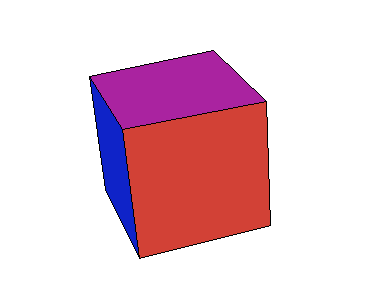
\includegraphics[width=0.8\textwidth]{rotated_cube.png}
\end{center}
\section{Adding physics to the universe}
This section of the report details the process of creating physical phenomena in the universe, such as gravity, air resistance and friction. Before adding any of these accelerative processes, points must be linked to the obloids they belong to in such a way that they can read various properties of obloids, namely the velocity, the mass, and whether the object is on the ground or not.

\begin{lstlisting}
	vector<int> velocity = {0, 0, 0};
	int mass = 5;
	bool on_floor = false;
\end{lstlisting}
This will be achieved through the use of pointers: a reference to a memory address storing the relevant information. Each point will be assigned a "parent obloid" by reference, although this must be done by means of a function that assigns these references at runtime (the process cannot be done beforehand).

\begin{lstlisting}

/* Inside Obloid class definition */
void initialise_planes() {
	for (int m = 0; m < faces.size(); m++) {
		for (int n = 0; n < faces[m].points.size(); n++) {
			faces[m].points[m].parent_obloid = this;
			faces[m].points[m].assign_properties();
		}
	}
}

/* Declared in point class definition, but defined outside */
void Point::assign_properties() {
	mass = parent_obloid->mass;
	on_floor = &parent_obloid->on_floor;
	xVel = &parent_obloid->velocity[0];
	yVel = &parent_obloid->velocity[1];
	zVel = &parent_obloid->velocity[2];
}
\end{lstlisting}
Now, after running \verb|point.assign_properties()| for every point, the velocity of an obloid is linked to the velocity of the points that make up the obloid, and can be used to update the position of the point.
\newline
\newline
\newline
\begin{lstlisting}
void update() {
	/* Safeguards against null pointer */
	if (xVel) {
		abs_pos[0] += *xVel;
		abs_pos[2] += *zVel;

		if (on_floor) {
			abs_pos[1] += *yVel;
		}
	}

	screen_x = window_width * 0.5 + window_width * rel_pos[0] / (rel_pos[2] * tan(fov));

	screen_y = window_height * 0.5 + window_width * rel_pos[1] / (rel_pos[2] * tan(fov));	

}
\end{lstlisting}
\subsection{Gravity}
The strength of gravity in the universe will be set by a constant global variable, and will be added to all obloids that are not on the ground every event loop. Because the loop runs every 5 milliseconds, the gravitational constant will be different to 9.81, as it is on Earth. 
\newline
\newline
The actual values used here are not of great significance, as the aim is to produce accurate dynamics of projectile motion, and not necessarily to replicate projectile motion on Earth.

\begin{lstlisting}

const float GRAVITY = 0.4;
/* Dictates the minimum global y value ie. ground level */
const int FLOOR_Y = 100;

\end{lstlisting}

The gravitational acceleration will be implemented by adding \verb|GRAVITY| to each obloid's y velocity (taking y positive as down). There will also be a check to ensure that the obloid has not exceeded \verb|FLOOR_Y| included in the \verb|Point| definition.
\newpage
\begin{lstlisting}

/* Point method */
void update() {
	
	//Above code hidden

	/* Assigns value of on_floor, which can be read by parent obloid. */
	if (on_floor && abs_pos[1] > FLOOR_Y) {
		*on_floor = true;
	}
}

/* Obloid method */
void update_faces(HDC hdc) {
	
	if (on_floor) {
		velocity[1] = 0;

	}
	else if (mass && !on_floor) {
		velocity[1] += GRAVITY;
	}
			
	for (int f = 0; f < faces.size(); f++) {
		faces[f].update_points();
		faces[f].fill_plane(hdc);
	}
}

\end{lstlisting}
Obloids with a non-zero mass will now accelerate downwards until they hit the ground.

\subsection{Vertical Impact Mechanics}

By preserving momentum when colliding with the ground, obloids can be made to bounce according to Newton's law of Restitution, $ e = \frac{u}{v} $. Because the impulse acts upwards, perpendicular to the ground, only the y velocity is altered in the collision. First, a coefficient of restitution will be included in the list of properties for obloids. This will be used to calculate the speed of rebound for each collision with the ground.
\newpage
\begin{lstlisting}

/* Obloid definition */
float restitution = 0.8;

void update_faces(HDC hdc) {
	
	if (on_floor) {
		if (abs(velocity[1] < 0.2) {	
			velocity[1] = 0;
		}
		else {
			velocity[1] = -restitution * velocity[1];
		}

	}
	else if (mass && !on_floor) {
		velocity[1] += GRAVITY;
	}
			
	for (int f = 0; f < faces.size(); f++) {
		faces[f].update_points();
		faces[f].fill_plane(hdc);
	}
}

\end{lstlisting}

By adding a test to see if the velocity falls below a certain threshold, infinite bouncing is prevented by setting the velocity to zero.

\subsection{Air Resistance}
With all three velocity components separated, adding realistic air resistance is simplified. Assuming that air resistance follows a quadratic model \cite{airres}, the equations for drag force are as follows:

$$ D_x = \frac{1}{2}C_d \rho {v_x}^2 A_x  $$
$$ D_y = \frac{1}{2}C_d \rho {v_y}^2 A_y  $$
$$ D_z = \frac{1}{2}C_d \rho {v_z}^2 A_z  $$

Where $C_d$ is a coefficient (typically determined by experiemnt), $\rho$ is the density of the medium, $v_{x, y, z}$ are the x, y, z components of the velocity and $A$ is the surface area of the face experiencing the drag force. For now, air will remain at a constant density, and can be combined with the coefficient $C_d$ to create a single parameter determining how much the air resistance affects the motion of the obloid.
\newline
\newline
First, all of these properties must be defined for each obloid. The drag force will be represented as an array, as will the 3 different surface areas for the obloid's faces.
\begin{lstlisting}
/* Obloid definition */
int width = abs(trf.abs_pos[0] - tlf.abs_pos[0]);
int height = abs(trf.abs_pos[1] - brf.abs_pos[1]);
int breadth = abs(trf.abs_pos[2] - trb.abs_pos[2]);

float air_resistance_const = 0.01;
vector<int> face_areas = { width * height, 
						  	  width * breadth, 
						  	  height * breadth };
vector<float> drag_force = { 0, 0, 0 };
\end{lstlisting}
Each event loop, the drag force will be recalculated and applied to each component of the velocity, causing decceleration in all three axes:

\begin{lstlisting}
void update_faces{HDC hdc) {
	if (on_floor) {
		//Code hidden
	}
	else if (mass && !on_floor) {
		velocity[1] += GRAVITY;	
	
		for (int d = 0; d < 3; d++) {
			drag_force[d] = pow(velocity[d], 2) * air_resistance_const * faces_areas[d];
			if (velocity[d] < 0.2) {
				velocity[d] = 0;
			}
			else {
				velocity[d] -= drag_force[d] / mass;
			}
		}
	}
}
\end{lstlisting}
Again, there is a threshold for each component of the velocity, to prevent issues with very small velocities.
\newpage
\subsection{Friction}
Friction will be the final physical phenomenon included in the engine. Because there are currently no inclined planes in the engine, and no active forces in the x-z plane (ie. no forces causing positive horizontal acceleration), friction can simply be modelled as a constant deceleration of objects in contact with the ground. The deceleration will only affect x and z velocity.
\newline
\newline
A coefficient of friction (typically denoted $\mu$) will be specified in each obloid's properties, and will act in the opposite direction to the x and z velocity:
\begin{lstlisting}
/* Obloid definition */
float friction = 0.06;

void update_faces{HDC hdc) {
	if (on_floor) {
	
		/* Handles rebounds */
		if (abs(velocity[1] < 0.2) {	
			velocity[1] = 0;
		}
		else {
			velocity[1] = -restitution * velocity[1];
		}
		
		/* Applies friction */
		if (abs(velocity[0]) < 0.2) {
			velocity[0] = 0;
		}
		else {
			velocity[0] -= sgn(velocity[0]) * friction;
		}
		if (abs(velocity[2]) < 0.2) {
			velocity[2] = 0;
		}
		else {
			velocity[2] -= sgn(velocity[2]) * friction;
		}
	}
	else if (mass && !on_floor) {
		//Code hidden
	}
}
\end{lstlisting}

With friction implemented, all of the physical mechanics required for simluating projectile motion have been added.

\newpage
\section{Conclusion and Evaluation}
With the development of the engine complete for the purposes of this project, there are some pictures included below demonstrating the physics created in the previous section:
\newline
\newline
\newline
Rebounds with each frame shown:
\newline
\includegraphics[width=1\textwidth]{projectile_motion_2.png}
\newline
\newline
\newline
Rebounds with only the trace and the final position shown:
\newline
\includegraphics[width=1\textwidth]{projectile_motion_4.png}
\newline
As you can see in both of these images, the bounces become successively lower, with subsequent collisions with the ground, demonstrating that the impact mechanics are functioning correctly.
\newline
Furthermore, as shown by the trace in the second image, the bounces are not symmetrical, indicating the effect of air resistance. Note that the effect of air resistance has been exaggerated for visibility, and realistically would have a much lesser effect.
\newpage
Rebounds followed by slide:
\newline
\newline
\includegraphics[width=1\textwidth]{projectile_motion_5.png}
\newline
As can be seen in this image, there is a lower coefficient of restitution, resulting in fewer bounces, and a longer contact with the ground at the end. While difficult to demonstrate with a static image, the cube decelerates until stopping, once it is continuously in contact with the floor. This indicates that friction is working as intended.
\newline
\newline
\newline
It is worth considering some limitations of the model. There is currently no implementation of moments, which limits the ability of the model to represent phenomena such as spin and oblique impacts. Furthermore, a more mathematically elegant solution to how forces are applied to obloids (ie. with the use of a matrix transformation) could allow for some more advanced mechanics techniques, namely improving the air resistance model such that turbulence can be accounted for. The Navier-Stokes equations 
\cite{turb}
could be used to implement vortices for example, allowing for even more advanced projectile motion.
\newline
\newline
While there are many areas in which the engine could be further developed, the images above, as well as the program running in real-time give an accurate model of projectile motion. If you would like to see the engine running in real time, the whole project is available to download and run on \href{https://github.com/maximwebb/3D-engine}{\color{blue} on Github}\color{black}.

\newpage
\begin{thebibliography}{2}
\bibitem{airres}
Drag Equation
\\\texttt{https://www.grc.nasa.gov/WWW/K-12/airplane/drageq.html}
\bibitem{turb}
Turbulence, J. M. McDonough
\\\texttt{http://www.engr.uky.edu/~acfd/lctr-notes634.pdf}
\end{thebibliography}
\end{document}